\section{Search Methodology}
\subsection{Position and move operations}
The native engine packs squares and moves into integers and represents each wall orientation with one 64-bit mask. Precomputed masks encode blocked edges, crossings, and same-orientation overlap. Make/unmake updates pawns, reserves, wall masks, side to move, and an incremental Zobrist key. TT entries also retain complete packed-position verification, preventing a hash collision from returning another position's score.

Move generation is staged. Pawn actions and structurally available walls are generated cheaply; expensive path work is delayed until alpha--beta actually searches a candidate. A retained route certificate can prove that a wall leaves a path intact. If the wall intersects that certificate, direct bitboard breadth-first search recomputes reachability and distance. The measured funnel is shown in \cref{fig:path-funnel}.

\begin{figure}[t]
\centering
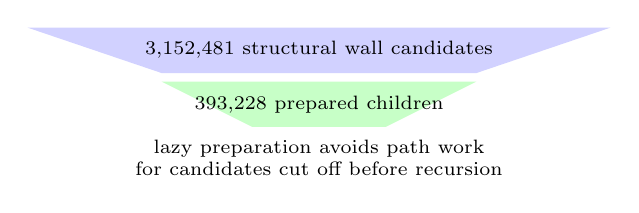
\begin{tikzpicture}[x=1cm,y=0.72cm,font=\scriptsize]
\fill[blue!18] (0,2) -- (7.4,2) -- (5.7,1.2) -- (1.7,1.2) -- cycle;
\fill[green!22] (1.7,1.05) -- (5.7,1.05) -- (4.55,0.25) -- (2.85,0.25) -- cycle;
\node at (3.7,1.62) {3,152,481 structural wall candidates};
\node at (3.7,0.65) {393,228 prepared children};
\node[align=center] at (3.7,-0.3) {lazy preparation avoids path work\\for candidates cut off before recursion};
\end{tikzpicture}

\caption{A diagnostic opening search observed millions of structural wall candidates but prepared only the candidates reached before a cutoff.}
\label{fig:path-funnel}
\end{figure}

\subsection{Tree search and verification}
Production search uses iterative deepening, fail-soft negamax, alpha--beta bounds, principal-variation search, aspiration windows, mate-distance bounds, TT ordering, history, killers, and selective late-move reductions. A reduced search that can improve alpha is re-searched at the required depth and window. Exact left--right root symmetry removes only actions whose scores are mathematically identical under reflection.

At every completed hybrid iteration, the main lane reports \mainDepth{} and the maximum extended line reports \selDepth. The verifier reports \verifiedDepth{} only after all required legal root actions complete. Root positions with no remaining walls can invoke an exact retrograde solver over the fixed-topology pawn-and-turn graph and return a replayable outcome and distance.

\subsection{Production versus experiments}
The production experiment mask is \ProductionMask. Topology caches, alternative histories, strategic evaluation, additional pruning, learned models, canonical TT storage, and all-shortest-route candidates remain individually versioned experiments. Passing parity proves only that an experiment respects the tested rules; it does not promote the experiment. Fixed-node quality, fixed-time performance, tactical regret, and paired strength evidence are separate gates.
